

\begin{frame}
\frametitle{Background measurements (Run IV, 2018)} 
\begin{figure}
  \begin{center}
    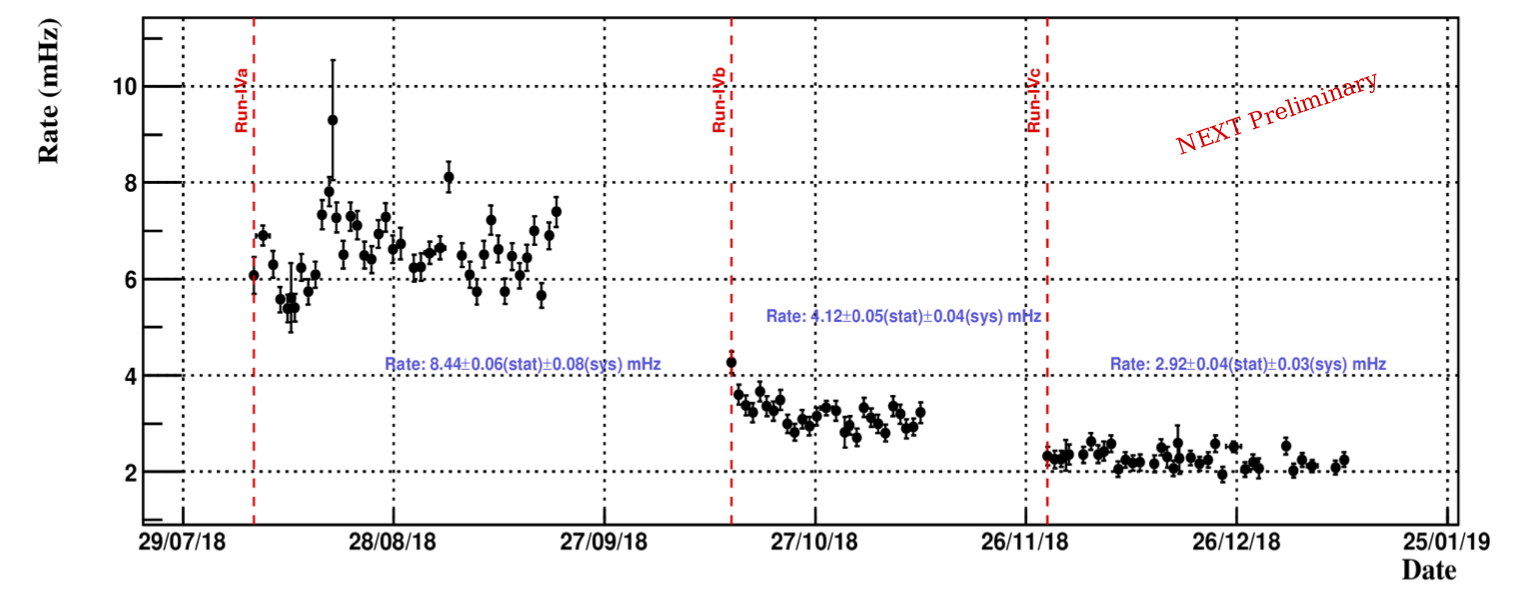
\includegraphics[scale=0.4]{moriond/run4_fid_rate.png}
    \caption{Fiducial background rate for Run IV (2018) as a function of data taking calendar day. Vertical dashed lines mark the times where Run-IVa, Run-IVb and Run-IVc started.}
    \label{fig:rate}
  \end{center}
\end{figure}
\begin{itemize}
\item {\bf Run IVa}. No radon free air, no inner shielding. 
\item {\bf Run IVb}. Radon free air. 
\item {\bf Run IVc}. Radon free air and inner shielding
\end{itemize}
\end{frame}

\begin{frame}
\frametitle{Background composition} 
\begin{figure}
  \begin{center}
    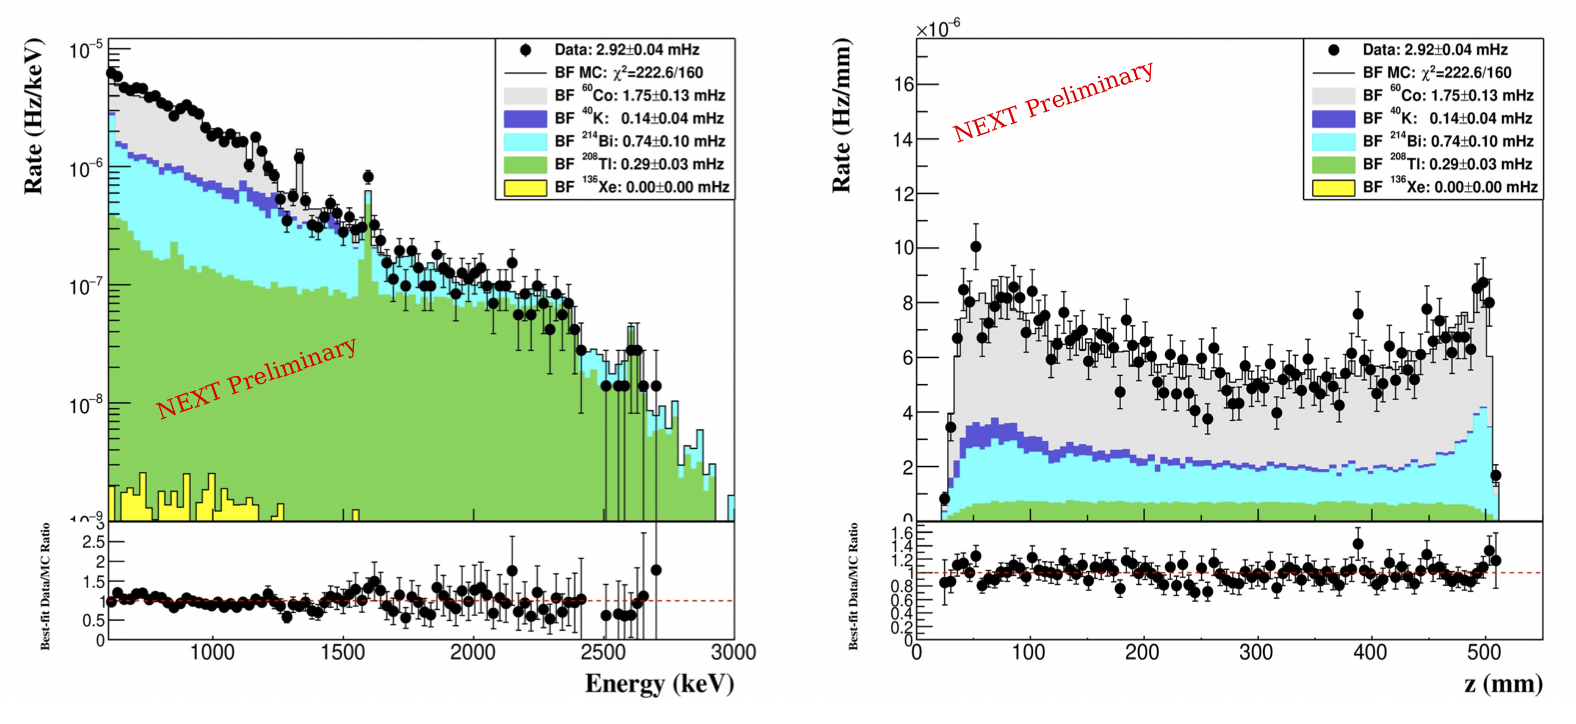
\includegraphics[scale=0.4]{moriond/bkgnd_fit.png}
    \caption{Contribution of the dominant background isotopes to \NEW\ radioactive budget.}
    \label{fig:rate}
  \end{center}
\end{figure}
\begin{itemize}
\item Notice, only \BI\ and \TL\ relevant for \bbonu\ searches. 
\end{itemize}
\end{frame}

%\begin{frame}
%\frametitle{Background composition (Run IV)} 
%\begin{figure}
%  \begin{center}
%    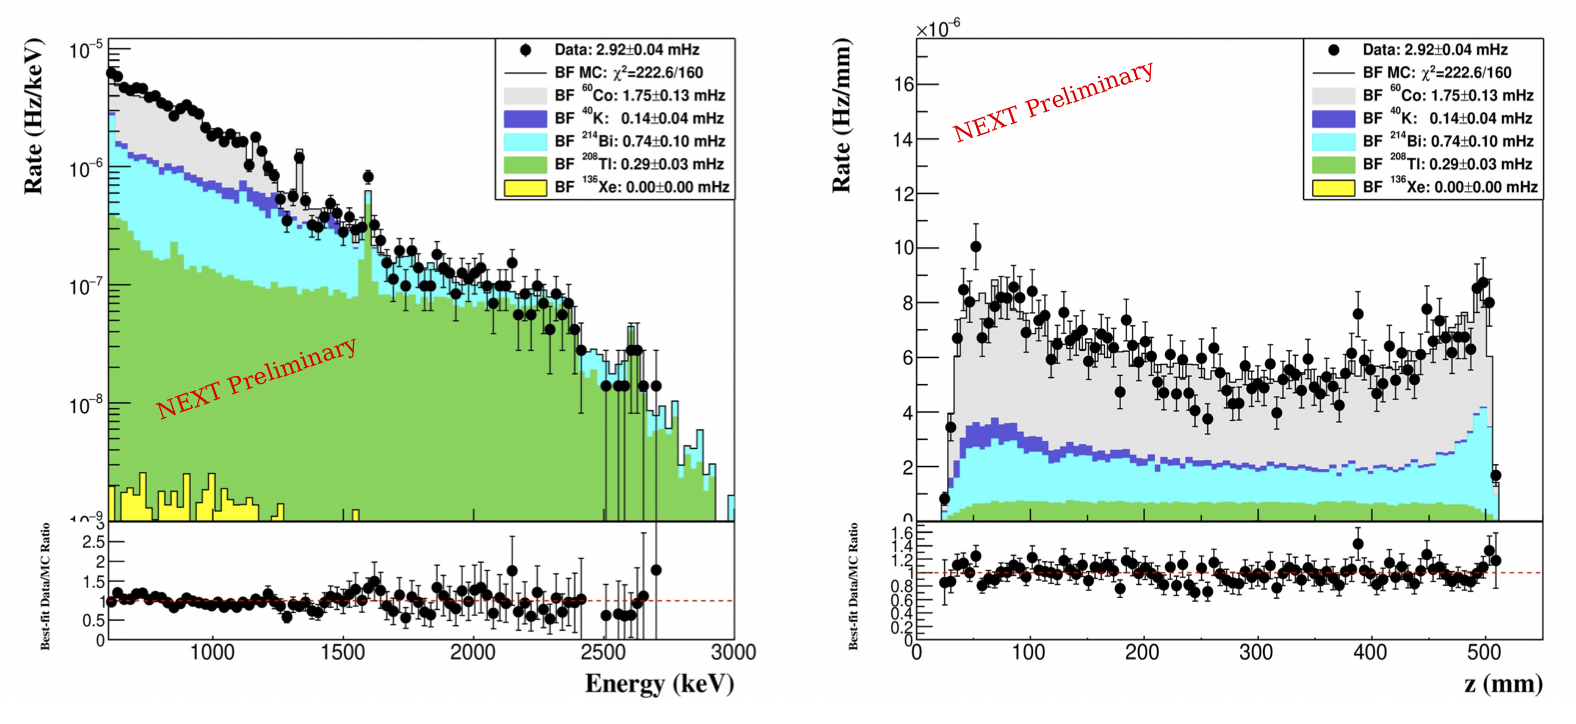
\includegraphics[scale=0.4]{moriond/bkgnd_fit.png}
%    \caption{Contribution of the dominant background isotopes to \NEW\ radioactive budget.}
%    \label{fig:rate}
%  \end{center}
%\end{figure}
%\begin{itemize}
%\item Notice, only \BI\ and \TL\ relevant for \bbonu\ searches. 
%\end{itemize}
%\end{frame}


\begin{frame}
\frametitle{Run V (enriched xenon)} 
\begin{figure}
  \begin{center}
    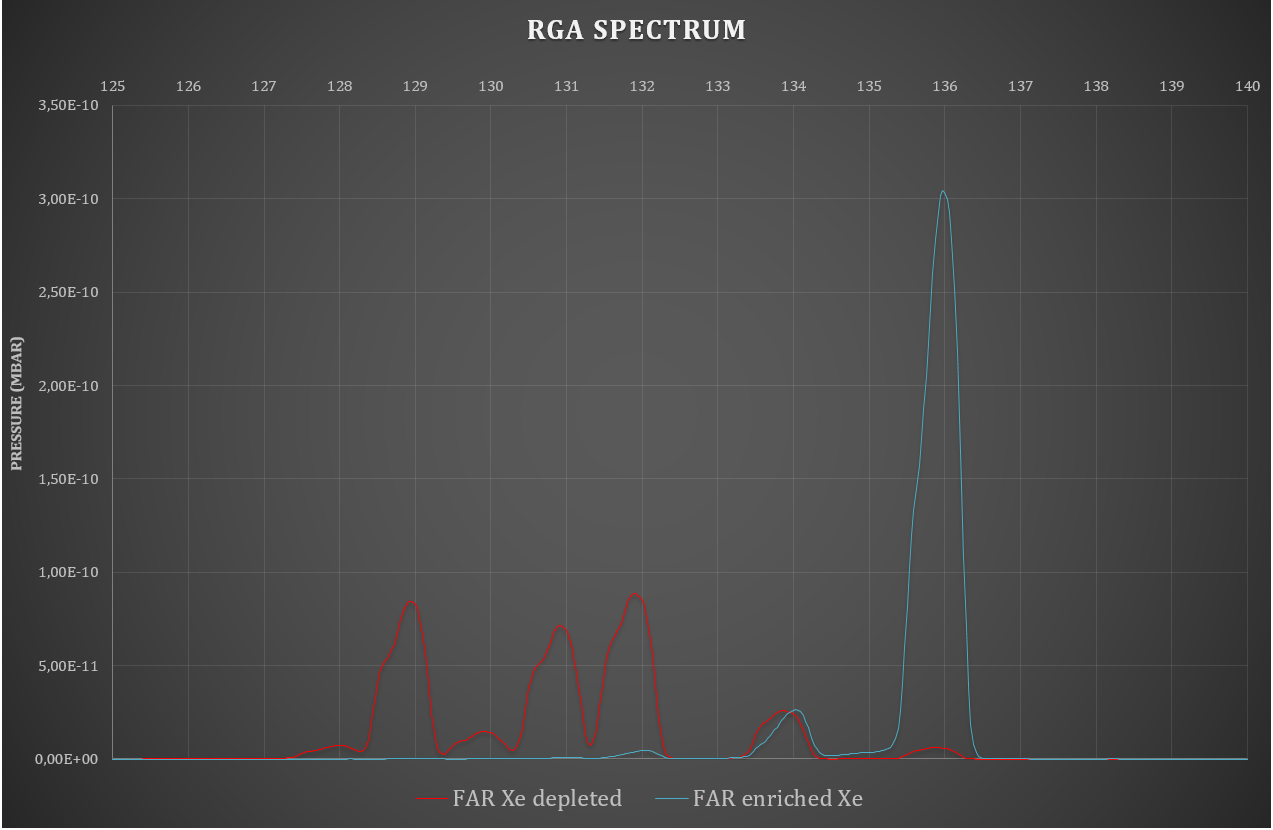
\includegraphics[width=0.9\textwidth]{moriond/XeEnriched.png} 
    \caption{We really have enriched xenon...}
    \label{fig:exe}
  \end{center}
\end{figure}
\end{frame}

\begin{frame}
\frametitle{Measurement of \bbtnu\ mode (Run V)} 
\begin{figure}
  \begin{center}
    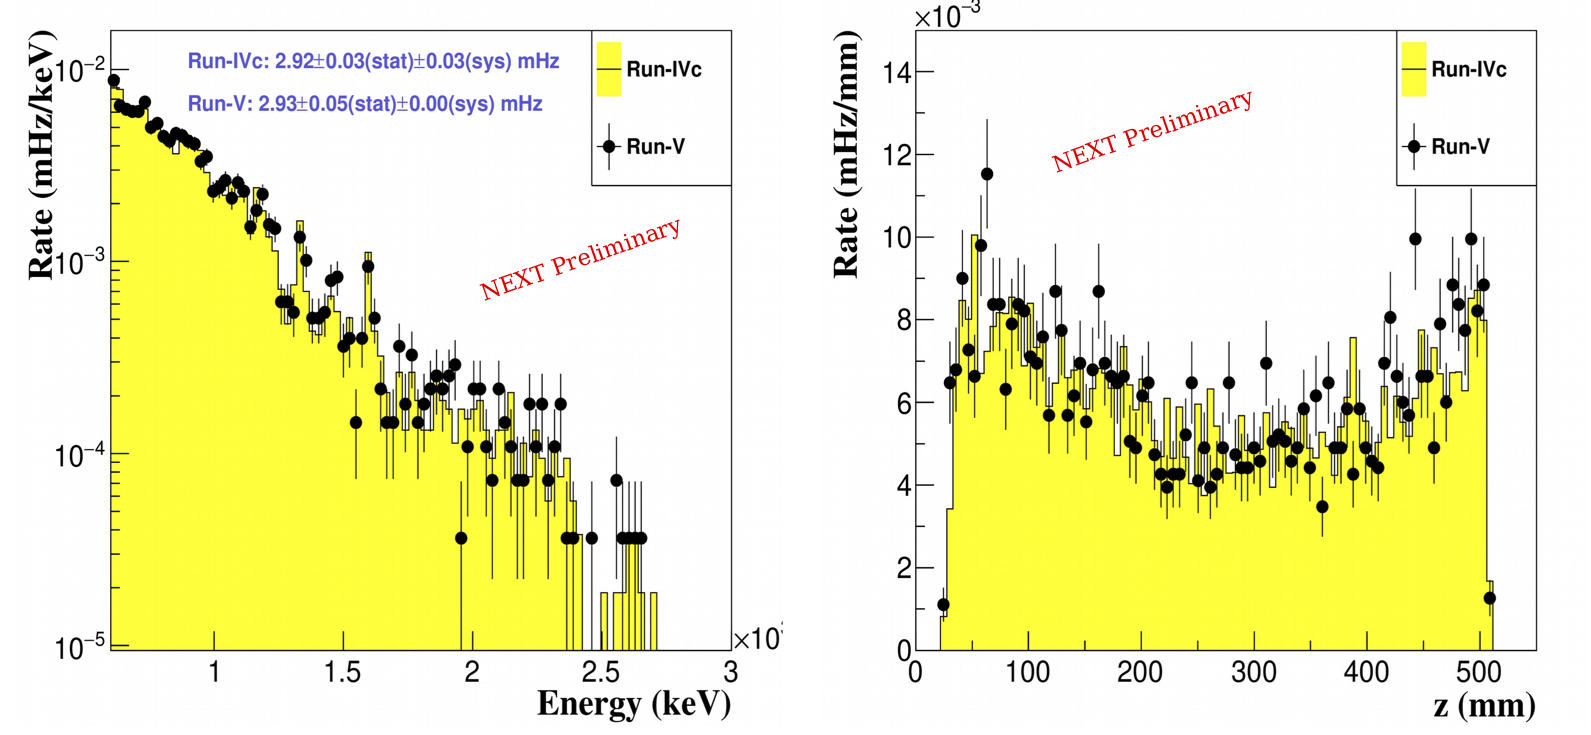
\includegraphics[scale=0.4]{moriond/run5_spectra.png}
    \caption{Energy spectra, Run V.}
    \label{fig:rate}
  \end{center}
\end{figure}
\begin{itemize}
\item Notice, Run V just started (15 days taking data with enriched xenon). 
\item Will run until the end of the year to provide a measurement of \bbtnu\ lifetime.  
\end{itemize}
\end{frame}

\begin{frame}
\frametitle{High energy spectrum with topological cuts} 
\begin{figure}
  \begin{center}
    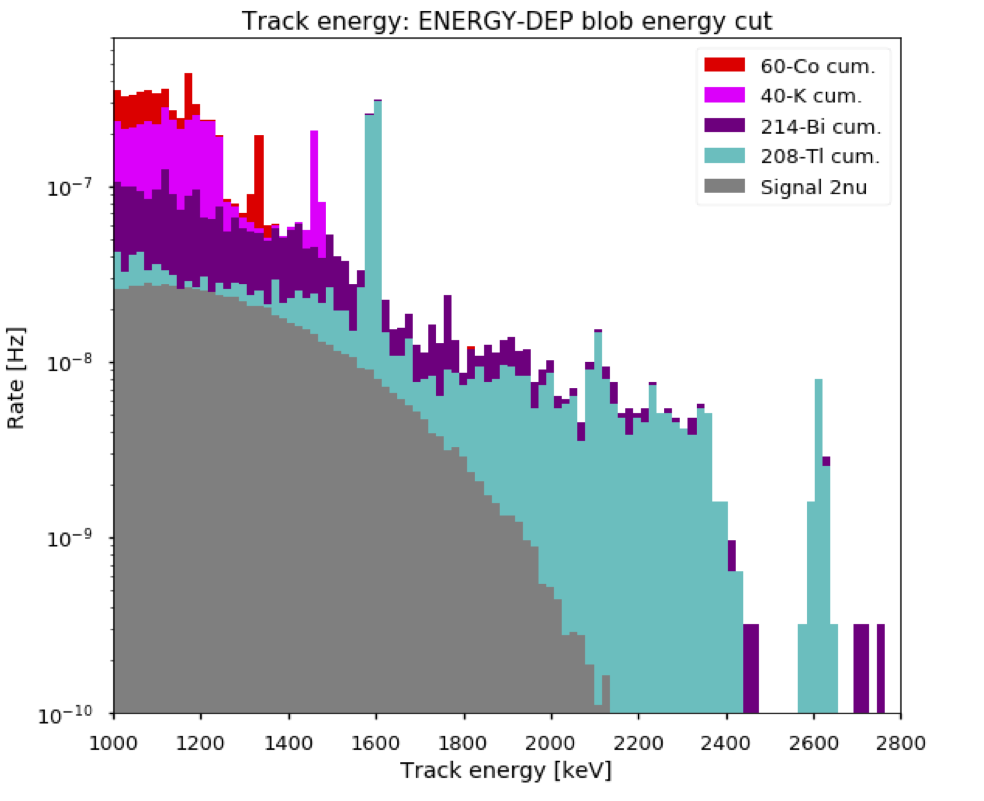
\includegraphics[scale=0.35]{moriond/new_with_topo_log.png}
     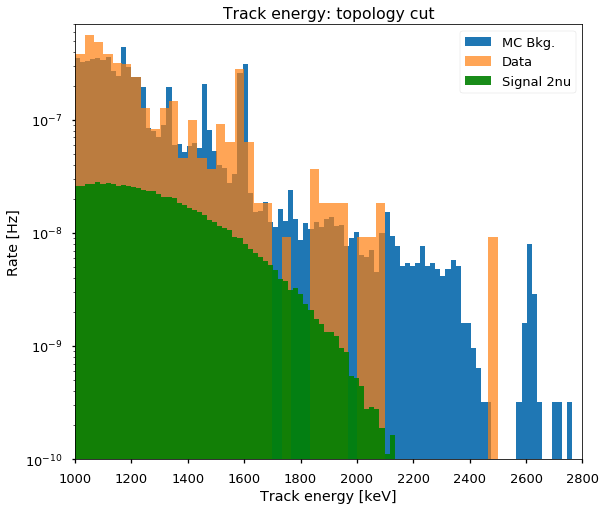
\includegraphics[scale=0.30]{moriond/energy_spectrum_total.png}
    
    \caption{Energy spectra with topological cuts data and MC. }
    \label{fig:rate}
  \end{center}
\end{figure}
\begin{itemize}
\item Topological cut cleans high energy region where signal is expected (notice the hole). 
\item One candidate event found in the data by basic topological analysis (visual inspection shows badly reconstructed single electron event).  
\end{itemize}
\end{frame}





%\begin{frame}
%\begin{table}[!htb]
%\caption{\label{tab:rate} Run-IV background rates for events with energy above 600 keV.}
%\begin{center}
%\begin{tabular}{ccc}
%\hline
%Run period & Inclusive rate (mHz) & Fiducial rate (mHz) \\ \hline
%Run-IVa    &    14.85$\pm$0.06    &  7.05$\pm$0.05                  \\ 
%Run-IVb    &     8.77$\pm$0.06    &  3.70$\pm$0.04                  \\
%Run-IVc    &     7.03$\pm$0.10    &  2.72$\pm$0.06                   \\ \hline
%\end{tabular}
%\end{center}
%\end{table}
%\end{frame}
%
%\begin{frame}
%\begin{figure}
%  \begin{center}
%    \includegraphics[scale=0.6]{img2/RateTime_eFidSel_RunIVabc.pdf}
%    \caption{Fiducial background rate as a function of data taking calendar day. Vertical dashed lines mark the times where Run-IVa, Run-IVb and Run-IVb started.}
%    \label{fig:rate}
%  \end{center}
%\end{figure}
%\end{frame}
%
%\begin{frame}
%\begin{figure}
%  \begin{center}
%    \includegraphics[scale=0.40]{img2/RunIVabc_energy.pdf}
%    \caption{Fully corrected energy spectra of the fiducial background samples collected during Run-IV.}
%    \label{fig:energy}
%  \end{center}
%\end{figure}
%\end{frame}
%
%\begin{frame}
%\frametitle{Run-IVa} 
%\begin{itemize}
%\item The background rate in Run-IVa has decreased by a factor of 1.7 with respect to the earlier pilot background run taken in 2017 (Run-II), despite the pressure increase from 7.2 to 10 bar.
%\item This background rate reduction confirms the expected improvement in detector radiopurity introduced by the replacement of the field cage resistor chain and the PMT bases in early 2018.
%\item However, the rate variations in time (not consistent with statistical fluctuations) observed for Run-IVa in Fig.~\ref{fig:rate} are a clear indication of a time-dependent background source, thereby not related to radio-impurities of the detector materials.
%\item The analysis of the correlation of the background rate with the level of airborne radon at the LSC has allowed to conclude that such variations are due to a significant contribution of $^{222}$Rn decays within the volume of the lead castle.  
%\item Using the radon activity data provided by the Alphaguard detector, the correlation is quantified in Fig.~\ref{fig:rncorr} by means of a linear fit. From this fit, an expectation of the fiducial background rate in NEXT-White for a zero-Rn-activity is derived: 3.65$\pm$0.37 mHz.    
%\end{itemize}
%\end{frame}
%
%\begin{frame}
%\begin{figure}
%  \begin{center}
%    \includegraphics[scale=0.64]{img/RnCorr_eFidSel.eps}
%    \caption{Airborne radon activity versus Run-IVa fiducial background rate. A linear fit extrapolation to zero-Rn-activity yields an expected background rate of 3.65$\pm$0.37 mHz.}
%    \label{fig:rncorr}
%  \end{center}
%\end{figure}
%\end{frame}
%
%\begin{frame}
%\frametitle{Run-IVb} 
%\begin{itemize}
%\item The effect of the RAS in Run-IVb is clearly visible in Fig.~\ref{fig:rate} and Fig.~\ref{fig:energy}. After a few-days period where the background rate decreases as the remaining $^{222}$Rn inside the castle decays, the fiducial background rate becomes stable when a reduction of a factor of 1.9 with respect to Run-IVa is reached.
%\item The comparison of the energy spectra in Run-IVa and Run-IVb around 1700 keV (1764 keV $\gamma$-line of $^{214}Bi$) positively identifies this reduction as due to $^{222}$Rn.
%\item The consistency between the background rate measurement in Run-IVb (3.70$\pm$0.04 mHz) and the zero-Rn-activity background extrapolation from Run-IVa (3.65$\pm$0.37 mHz) implies that the RAS allows for a virtually airborne-Rn-free operation of the NEXT-White detector. 
%\end{itemize}
%\end{frame}
% 
% \begin{frame}
%\frametitle{Run-IVc} 
%\begin{itemize}
%\item The main goal of the ILC installed between Run-IVb and Run-IVc is to provide further shielding to background contributions coming from the outer lead castle volume. 
%\item In particular, the radioactivity from the castle structure paint is a major candidate to be suppressed.
%\item As shown, Fig.~\ref{fig:rate} and Fig.~\ref{fig:energy}, the Run-IVc data already indicates a reduction in the fiducial background rate of about 40\% despite the current limited statistics. 
%\item This implies that Run-IVa and Run-IVb suffer from a significant contribution of external backgrounds not related to airborne radon ($\sim$1 mHz). The main candidate source of this external background is the castle structure paint.
%\item Beyond the reduction of overall background rate, it is worth remarking the stability of the rate over time, presented in Fig.~\ref{fig:ratec}. 
%\end{itemize}
%\end{frame}
%  
% \begin{frame}
%\begin{figure}
%  \begin{center}
%    \includegraphics[scale=0.60]{img2/Rate_eFidSel_time.pdf}
%    \caption{Run-IVc fiducial background rate as a function of calendar day. A linear fit shows the compatibility with a flat distribution. The vertical dashed lines marks the time of the different sub-runs taken so far.}
%    \label{fig:ratec}
%  \end{center}
%\end{figure}
%\end{frame}
%%
%%
%\begin{frame}
%\frametitle{Background model} 
%\begin{itemize}
%\item The expected background budget in NEXT-White is derived from a detailed background model accounting for different isotopes and detector volumes. 
%\item The model relies on the extensive radiopurity measurements campaign conducted by the NEXT collaboration. Up to 41 detector materials have been considered, screening their $^{214}$Bi, $^{208}$Tl, $^{40}$K and $^{60}$Co contributions.
%\item According to these measurements, a full GEANT4-based Monte-Carlo simulation has been performed. The screened materials are associated to 19 GEANT-4 volumes describing the components of the NEXT-White detector. These volumes can be grouped in 6 different detector subsystems: active volume, energy readout plane, tracking readout plane, field cage, pressure vessel and shielding. Accounting for the 4 isotopes considered, the background model consists of 76 (19$\times$4) background sources. In addition, the contribution from the $\beta\beta2\nu$ of $^{136}$Xe, whose fraction in the depleted Xe in use is 2.86\%, is also incorporated to the model. Overall, 10$^{11}$ background events have been simulated, corresponding to an exposure of 6.35 year. 
%\end{itemize}
%\end{frame}
%
%\begin{frame}
%\begin{itemize}
%\item The simulated background events are first processed to mimic the electronic effects (readout, shaping, noise, ...), so the corresponding raw waveforms can be already compared to the ones collected by the DAQ system. Then, the Monte-Carlo events are passed through the same reconstruction and corrections steps as described for real data. Finally, the fiducial selection is applied. 
%\item The resulting background energy spectra are shown in Fig.~\ref{fig:bgmodel}, in terms of the different isotopes contribution (right) and of the different subsystem contributions (left). Since the background model includes neither the contribution of external airborne-Rn nor the ILC, it is to be compared with the data taken in Run-IVb. According to the described model, the expected fiducial background rate in Run-IVb is 1.699$\pm$0.003 (stat) mHz.
%\item An updated background model is being currently built considering the ILC, thus to be compared with the Run-IVc data. In particular, the $^{214}$Bi, $^{208}$Tl, $^{40}$K and $^{60}$Co contributions of the ILC bricks, as well as the $^{214}$Bi and $^{208}$Tl contribution of the ILC steel structure, are accounted for. In addition, a new contribution from Rn-induced $^{214}$Bi on the cathode surface is included, according to the measurements performed with Run-II data. Overall, the updated model consists of 84 background sources. So far, 1.5 million events (corresponding to 5.48 years) have been simulated and are currently being processed in the reconstruction stage. 
%\end{itemize}
%\end{frame}
%
%\begin{frame}
%\begin{figure}
%  \begin{center}
%    \includegraphics[scale=0.3]{img/MCE.eps}
%    \includegraphics[scale=0.3]{img/MCEVol.eps}
%    \caption{MC background model for Run-IVb: fiducial background rate as a function of the energy. Right: contributions from the 4 isotopes considered. Left: contributions from the 6 subsystems considered, accounting for 19 GEANT-4 volumes.}
%    \label{fig:bgmodel}
%  \end{center}
%\end{figure}
%\end{frame}
%
%\begin{frame}
%\frametitle{Data-Monte Carlo comparison} 
%\begin{itemize}
%\item The comparison of the background model described previously with the Run-IVb data is presented in the left panel of Fig.~\ref{fig:bgfit}. While the different gamma lines are well reproduced in the model, the overall data rate (3.70$\pm$0.04) deviates from the expectation (1.699$\pm$0.003 mHz) by a factor $\sim$2.2 It is worth noticing that a good fraction of such a discrepancy is due to external backgrounds that have been suppressed in Run-IVc with the ILC. {\em This consideration, along with the missing contribution of Rn-induced $^{214}$Bi on the cathode in the current model, allows to foresee a good matching between the data and the model in the near-future Run-IVc comparison}. 
%\item In order to tune the Run-IVb background model so it matches the data, an effective fit has been performed. The fit consists of the minimization of a maximum extended likelihood, considering both the energy and the z-coordinate distribution of the background events, as well as three effective background volumes in the model. The three volumes account for all materials in the anode and cathode regions, and in any other region (ie, field cage, vessel, and shielding). The rationale for the definition of these effective volumes is to fully exploit the clear z-dependence observed in the background data. 
%\item The best-fit reproduces the energy spectrum, although yielding an overall scale factor of the expected rate of 2.19$\pm$0.15. 
%\end{itemize}
%\end{frame}
%
%\begin{frame}
%\begin{figure}
%  \begin{center}
%    \includegraphics[scale=0.30]{img/DataMCE_eFidSel_EZFit_3Vols.eps}
%    \includegraphics[scale=0.30]{img/DataMCEBF_eFidSel_EZFit_3Vols.eps}
%    \caption{Fiducial background energy spectra in Run-IVc. Data (black dots) are superimposed to the background model expectation (solid histograms), for which the different isotopes contributions are shown. Left: expectation from nominal background model. Right: expectation from best-fit to data, were the displayed best-fit values correspond to the scale factor of each isotope with respect to the nominal model.}
%    \label{fig:bgfit}
%  \end{center}
%\end{figure}
%\end{frame}
%
%\begin{frame}
%\begin{figure}
%  \begin{center}
%    \includegraphics[scale=0.30]{img/DataMCZBF_eFidSel_EZFit_3Vols.eps}
%    \includegraphics[scale=0.30]{img/DataMCRBF_eFidSel_EZFit_3Vols.eps}
%    \caption{Fiducial background spatial distribution in Run-IVc. Data (black dots) are superimposed to the best-fit background model expectation (solid histograms), for which the different isotopes contributions are shown. Left: z distribution. Right: radial distribution. The displayed best-fit values correspond to the scale factor of each isotope with respect to the nominal model.}
%    \label{fig:zrbgfit}
%  \end{center}
%\end{figure}
%\end{frame}
%
